Perimeter-defense problems model scenarios where the interior of a region must be defended against a set of incoming attacks.
%
With a team of defenders (i.e., mobile robots and/or agents) located on the perimeter of a given region, an attack is considered successfully intercepted if at least one defender is present at the attack location when the attack happens. 
%
This problem finds broad applications, including the protection of endangered wildlife \cite{haksar2020spatial}, aerial defense \cite{lykou2020defending, lee2020perimeter}, and border security \cite{agmon2008multi, fengyu2020optimally}, to list a few. 

The study of perimeter defense problems finds some of its origins in target guarding problems \cite{rufus1965}, a classical pursuit-evasion game studying the strategies of multiple defenders to guard a static region.
%
In \cite{shishika2018local}, the target-guarding problem was first specialized to produce perimeter defense in which the perimeter is the target to be guarded, and defenders can only move on the perimeter. 
%
Various methods have been developed, including region decomposition \cite{shishika2018local}, assignment or matching-based algorithm \cite{shishika2020cooperative}, network flow formulation \cite{chen2021optimal}, and coverage control-based method \cite{macharet2020adaptive}.

Perimeter-defense problems may also be considered a variant of the reach-avoid game between two parties, where one party tries to send as many attackers to a region the other party must defend \cite{rufus1965}. 
%
Studies of the reach-avoid game usually apply specific case analysis, which suffers from the exponential increase in time complexity and size of state space as the number of attackers increase \cite{margellos2011hamilton, zhou2012general, yan2018reach}. 
%
Recent work leans toward adopting maximum matching or assignment frameworks from graph theory to address this problem for multiple defenders \cite{chen2014path, chen2014multiplayer, yan2019matching}.

% The target-guarding and reach-avoid games are usually categorized both in pursuit-evasion games. 

In this work, we study perimeter-defense problems under a perfect information assumption that the attackers' attack time and locations on the perimeter are known as soon as attackers appear. The assumption is adopted in several recent related research including \cite{adler2022role, macharet2020adaptive}.
%
The particular emphasis of our work is on the more challenging case of heterogeneous defenders, where the defenders have different speeds in responding to incoming attacks. 
%
We denote the problem as \emph{boundary-defense with heterogeneous defenders} or \prob.\footnote{We use \emph{boundary} instead of \emph{perimeter} since perimeter generally refers to the 1D boundary of a 2D geometry shape. 2D hemisphere has been examined in \cite{lee2020perimeter} for constraining defender.}
%
The heterogeneous setting for perimeters is first carefully investigated in \cite{adler2022role}, which carried out the detailed structural study and introduced an algorithm based on dynamic programming (DP) \cite{cormen2022introduction} for handling infinite horizon attacking sequences, focusing mostly on two defenders. 

\begin{figure}[t]
    \centering
    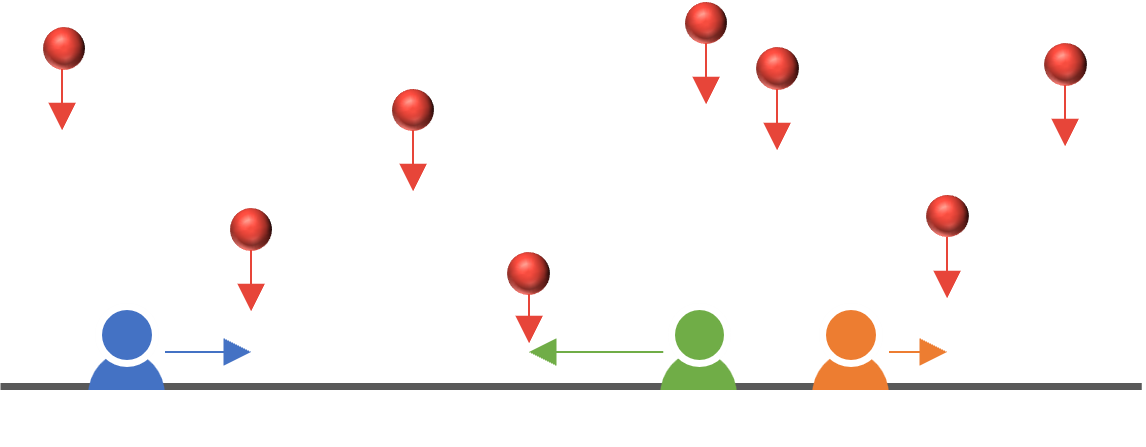
\includegraphics[width=1\linewidth]{chapters/bd/fig/bdhd.png}
    \vspace{-6mm}
    \caption[Illustration of the problem of boundary defense with heterogeneous defenders]
    {Illustration of the problem of boundary defense with heterogeneous defenders, where multiple defenders with different capabilities must do their best to intercept incoming attacks (signified as red balls moving downwards). The defenders are constrained to move on the boundary, which is a 1D perimeter in this case.}
    \label{fig:bd-bdhd}
    \vspace{-5mm}
\end{figure}
% \textbf{Related Work.}

%TODO: we focus on scalability (1) developed ILP algo (2) developed scalable algo (3) these algos enable us to carry out empirical studies including working with multiple topologies (can discuss hardness?)

The main contribution of our work lies in the development of efficient computational tools for and an empirical structural study of \prob. More specifically, 
\begin{itemize}[leftmargin=3.5mm]
\item We developed a network-flow formulation of \prob, leading to an exact method, based on integer linear programming (ILP), for solving the problem. The IP-based method is much more scalable than the DP-based method (which is only effective for no more than three defenders). 
% and the NP-hardness on the flow formulation of the problem  
\item Using the DP solution as a sub-routine, we developed a highly scalable heuristics method, called \emph{exhaustive defender pairing} (\ours), that runs in low polynomial time.  \ours is demonstrated to compute high-quality (in fact, often optimal or near-optimal) solutions. The design philosophy of \ours is of independent algorithmic interest. 
\item We further generalize our algorithms to apply to finite-horizon \prob (more challenging than infinite-horizon \prob), where only attacks whose attack time is within some $T$ time of hitting the boundary are revealed.
\item Utilizing the scalable algorithms developed in this work, we performed a thorough empirical study of the solution characteristics of \prob under various possible problem settings, including (1) different attack densities, (2) different defender speed distributions, and (3) different domain topology, i.e., $S^1$ (circle), $I = [0, 1]$ (unit interval), $S^2$ (sphere), and $I \times I$ (unit square). 
\end{itemize}

%2) a heuristic method based on exhaustive defender pairing that significantly reduces the computation time to solve perimeter defense problem with heterogeneous robot speed in a one-shot setting.
%3) a natural extension of the algorithm for the one-shot setting to the finite horizon continuous setting, where the robot team only know the attack events within a certain time frame in the future.

The rest of the chapter is organized as follows. 
In Sec.~\ref{sec:bd-preliminary}, we formulate the problems studied in this chapter and introduce the notations used. 
In Sec.~\ref{sec:bd-algorithm}, we describe the previous dynamic programming method in \cite{adler2022role}, 
and our ILP-based algorithms and \ours. 
We discuss the performance of our algorithms and solution characteristics of \prob under different settings in 
Sec.~\ref{sec:bd-evaluation}, 
and conclude with Sec.~\ref{sec:bd-conclusion}.
% The papers concludes with 

